\documentclass{article}
\usepackage{graphicx} % Required for inserting images
\usepackage{polski}
\usepackage[letterpaper,top=2cm,bottom=2cm,left=3cm,right=3cm,marginparwidth=1.75cm]{geometry}
\usepackage{amsmath}
\usepackage{graphicx}
\usepackage{algpseudocode}
\usepackage{array}
\usepackage{float}
\usepackage{pgfplots}
\pgfplotsset{compat=1.18}
\usepackage[colorlinks=true, allcolors=blue]{hyperref}

\title{Obliczenia naukowe lista 4}
\author{Stanisław Tomkowiak}

\begin{document}
\maketitle


\section*{Zadanie 1}
\subsection*{Opis zadania}
Napisać funkcję obliczającą ilorazy różnicowe.

\texttt{function ilorazyRoznicowe(x::Vector{Float64}, f::Vector{Float64})}
\subsubsection*{Dane wejściowe}
\begin{itemize}
    \item \texttt{x} – wektor długości $n + 1$ zawierający węzły $x_0, \ldots , x_n$
\texttt{x[1]=$x_0$,\ldots, x[n+1]=$x_n$}
    \item \texttt{f }– wektor długości $n + 1$ zawierający wartości interpolowanej
funkcji w węzłach $f(x_0), \ldots, f (x_n)$
\end{itemize}
\subsubsection*{Dane wyjściowe}
\begin{itemize}
    \item \texttt{fx} – wektor długości $n + 1$ zawierający obliczone ilorazy różnicowe
\[
\texttt{fx[1]}=f[x_0]
\]
\[
\texttt{fx[2]}=f [x_0, x_1],\ldots, \texttt{fx[n]}=f[x_0,\ldots , x_{n-1}], \texttt{fx[n+1]}=f [x_0,\ldots, x_n]
\]
\end{itemize}
\subsection*{Opis metody}
Kluczową częścią rozwiązania zadania jest użycie wzoru na ilorazy różnicowe wyższych rzędów:
\[ f[x_0] = f(x_0) \]
\[ f[x_i,x_j] = \frac{f(x_j)-f(x_i)}{x_j-x_i} \]
\[ f[x_i,x_{i+1},...x_{i+k}] = \frac{f[x_{i+1},...x_{i+k}]-f[x_i,...x_{i+k-1}]}{x_k-x_i}
\]
Łatwo zrozumieć sens działania algorytmu patrząc na poniższą tabelę.
\[
\begin{array}{cccccc}
$x_0$ & f[x_0] & f[x_0,x_1] & f[x_0,x_1,x_2] & f[x_0,x_1,x_2,x_3] \\
$x_1$& f[x_1] & f[x_1,x_2] & f[x_1,x_2,x_3] \\
$x_2$ & f[x_2] & f[x_2,x_3] \\
$x_3$ & f[x_3] \\
\end{array}
\]
Modyfikujemy wektor wejściowy \texttt{f} w trakcie działania algorytmu, stopniowo obliczając ilorazy różnicowe wyższych rzędów i zapisując je w odpowiednich pozycjach w \texttt{fx}. W pierwszej iteracji obliczamy wartości z drugiej kolumny tabeli, czyli \texttt{fx} staje się wektorem $[f[x_0], f[x_0,x_1], f[x_1,x_2], f[x_2,x_3]]$. W kolejnych iteracjach (dla $i = 2, 3, \dots$) obliczamy wyższe rzędy ilorazów różnicowych, zapisując je na kolejnych miejscach w \texttt{fx}.

W $i$-tej iteracji obliczamy wartości ilorazów różnicowych $f[x_0, \ldots, x_i], f[x_1, \ldots, x_{i+1}], \dots$, które odpowiadają kolejnej kolumnie tabeli. Ostatecznie, po zakończeniu wszystkich iteracji, wektor \texttt{fx} zawiera wyniki z pierwszego wiersza tabeli, od drugiej kolumny aż do końca. Są to ilorazy różnicowe wyższych rzędów, wyliczone zgodnie z podanym schematem.
\subsection*{Pseudokod}
\begin{algorithm}
\begin{algorithmic}[1]
\Function{IlorazyRóżnicowe}{$x$,$f$}

\State $fx \gets \text{kopiuj}(f)$
\State $len \gets \text{długość}(x)$

\For{$j \gets 1$ \textbf{to} $len$}
    \For{$i \gets len$ \textbf{downto} $j + 1$}
        \State $fx[i] \gets \frac{fx[i] - fx[i-1]}{x[i] - x[i-j]}$
    \EndFor
\EndFor

\State \Return $fx$
\end{algorithmic}
\end{algorithm}
\section*{Zadanie 2}
\subsection*{Opis zadania}
Napisać funkcję obliczającą wartość wielomianu interpolacyjnego stopnia $n$ w postaci Newtona $N_n(x)$ w punkcie $x = t$ za pomocą uogólnionego algorytmu Hornera, w czasie $O(n)$.

\texttt{function warNewton(x::Vector{Float64}, fx::Vector{Float64}, t::Float64)}
\subsubsection*{Dane wejściowe}
    \begin{itemize}
        \item \texttt{x} – wektor długości $n + 1$ zawierający węzły $x_0, \ldots , x_n$
\texttt{x[1]=$x_0$,\ldots, x[n+1]=$x_n$}
        \item \texttt{fx} – wektor długości $n + 1$ zawierający ilorazy różnicowe
\[
\texttt{fx[1]}=f[x_0]
\]
\[
\texttt{fx[2]}=f [x_0, x_1],\ldots, \texttt{fx[n]}=f[x_0,\ldots , x_{n-1}] \texttt{fx[n+1]}=f [x_0,\ldots, x_n]
\]
        \item \texttt{t} – punkt, w którym należy obliczyć wartość wielomianu
    \end{itemize}
\subsubsection*{Dane wyjściowe}
    \begin{itemize}
        \item \texttt{nt} – wartość wielomianu w punkcie $t$
    \end{itemize}
\subsection*{Opis metody}
Aby obliczyć wartość wielomianu interpolacyjnego stopnia n  w punkcie $x=t$ za pomocą uogólnionego algorytmu Hornera pokażmy jak wygląda taki wielomian w postaci Newtona $N_n(x)$:
\[
N_n(x) = f[x_0]+ f[x_0,x_1](x - x_0) + f[x_0,x_1,x_2] (x - x_0)(x - x_1) + \ldots + f[x_0,\ldots,x_n] (x - x_0)(x - x_1)\ldots(x - x_{n-1})
\]
Tak otrzymany wielomian kolejno zwijamy aby ograniczyć liczbę operacji:
\[
\[
N_n(x) = f[x_0] + (x - x_0) \left(f[x_0,x_1] + (x - x_1) \left(f[x_0,x_1,x_2] + \ldots + (x - x_{n-1})f[x_0,\ldots,x_n] \right)\right)
\]
W ogólności schemat rozwiązania wygląda tak:

\[ \omega_n(x) = f[x_0,\ldots,x_n] \]
\[ \omega_k(x) = f[x_0,\ldots,x_k] + (x-x_k) \cdot \omega_{k+1}(x) \]
\[ N_n(x) = \omega_0(x) \]

\subsection*{Pseudokod}
\begin{algorithm}

\begin{algorithmic}[1]
\Function{warNewton}{$x$, $fx$, $t$}
    \State $\text{len} \gets \text{length}(x)$
    \State $nt \gets fx[\text{len}]$
    \For{$i \gets \text{len} - 1, \dots, 1$}
        \State $nt \gets nt \cdot (t - x[i]) + fx[i]$
    \EndFor
    \State \Return $nt$
\end{algorithmic}
\end{algorithm}
\section*{Zadanie 3}
\subsection*{Opis zadania}
Znając współczynniki wielomianu interpolacyjnego w postaci Newtona $c_0 = f[x_0], c_1 =
f[x_0, x_1], c2 = f[x_0, x_1, x_2],\ldots, c_n= f[x_0,\ldots, x_n]$ (ilorazy różnicowe) oraz węzły $x_0, x_2,\ldots, x_n$ napisać funkcję obliczającą, w czasie $O(n^2)$, współczynniki jego postaci naturalnej $a_0,\ldots, a_n$ tzn. $a_nx^n+ a_{n-1}x^{n-1} +\ldots + a_1x + a_0$. 

\texttt{function naturalna(x::Vector{Float64}, fx::Vector{Float64}))}
\subsubsection*{Dane wejściowe}
    \begin{itemize}
        \item \texttt{x} – wektor długości $n + 1$ zawierający węzły $x_0, \ldots , x_n$
\texttt{x[1]=$x_0$,\ldots, x[n+1]=$x_n$}
        \item \texttt{fx} – wektor długości $n + 1$ zawierający ilorazy różnicowe
\[
\texttt{fx[1]}=f[x_0]
\]
\[
\texttt{fx[2]}=f [x_0, x_1],\ldots, \texttt{fx[n]}=f[x_0,\ldots , x_{n-1}] \texttt{fx[n+1]}=f [x_0,\ldots, x_n]
\]
    \end{itemize}
\subsubsection*{Dane wyjściowe}
\begin{itemize}
    \item \texttt{a} – wektor długości $n + 1$ zawierający obliczone współczynniki postaci naturalnej
\[
\texttt{a[1]}=a_0,\]
\[
\texttt{a[2]}=a_1,\ldots, \texttt{a[n]}=a_{n-1}, \texttt{a[n+1]}=a_n
\]    
\end{itemize}
\subsection*{Opis metody}
Aby obliczyć wartość współczynników wielomianu interpolacyjnego w postaci Newtona stopnia $n$ należy spojrzeć na wzór wielomianu postaci Newtona: 
\[
N_n(x) = f[x_0]+ f[x_0,x_1](x - x_0) + f[x_0,x_1,x_2] (x - x_0)(x - x_1) + \ldots + f[x_0,\ldots,x_n] (x - x_0)(x - x_1)\ldots(x - x_{n-1})
\]
Mamy go przekształcić do postaci:
\[
N_n(x) = a_0 + a_1 x + a_2 x^2 + \dots + a_n x^n
\]
Aby to osiągnąć podejmujemy takie kroki przed główną częścią algorytmu:
\begin{itemize}
    \item kopiujemy tablicę \texttt{fx} do tablicy \texttt{a}, to ona będzie przechowywać wyniki dla poszczególnych współczynników.
    \item sprawdzamy długość tablicy \texttt{fx} i zapisujemy ją do zmiennej \texttt{length}.
\end{itemize}
Algorytm działa iteracyjne od końca z zagnieżdżoną pętlą działającą od aktualnie rozpatrywanego $i=1$ do końca tablicy \texttt{a}. W każdym kroku algorytm wykonuje następujące kroki:
\begin{itemize}
    \item Dla każdego i, współczynnik a[i] jest aktualizowany według wzoru:
    \[
\texttt{a[i]}=\texttt{fx[i]}-\texttt{a[i+1]}*\texttt{x[i]},
\]
gdzie \texttt{a[i+1]} to współczynnik już obliczony w poprzednich iteracjach.
    \item Następnie, dla każdego $j$ od $i+1$ do $n-1$, aktualizowane są pozostałe współczynniki \texttt{a[j]}.
\end{itemize}
Po przejściu przez wszystkie iteracje algorytm zwraca tablicę \texttt{a}.

Ogólne założenie algorytmu polega na tym, że współczynniki są aktualizowane, uwzględniając poprzednie wartości. Dla każdej pary współczynników \texttt{a[i]} i \texttt{a[i+1]} wylicza się nową wartość \texttt{a[i]} jako różnicę między aktualną wartością funkcji \texttt{fx[i]} a poprzednim współczynnikiem \texttt{a[i+1]} pomnożonym przez \texttt{x[i]}. Zagnieżdżona funkcja służy natomiast do tego, aby uwzględnić wpływ węzłów poprzednich. W ten sposób, stopniowo, algorytm przekształca współczynniki z postaci Newtona na postać naturalną.
\subsection*{Pseudokod}

\begin{algorithm}
\caption{Przekształcenie wielomianu Newtona na postać naturalną}
\begin{algorithmic}[1]
\Function{naturalna}{x, fx}
\State \( \text{len} \gets \text{length}(fx) \)
\State \( a \gets fx \)

\For{ \( i \gets \text{len} - 1 \) \textbf{downto} 1 }
    \State \( a[i] \gets fx[i] - a[i+1] \cdot x[i] \)
    \For{ \( j \gets i + 1 \) \textbf{to} \text{len} - 1 }
        \State \( a[j] \gets a[j] - a[j+1] \cdot x[i] \)
    \EndFor
\EndFor

\State \Return a
\end{algorithmic}
\end{algorithm}
\section*{Zadanie 4}
\subsection*{Opis zadania}
Napisać funkcję, która zinterpoluje zadaną funkcję $f(x)$ w przedziale $[a, b]$ za pomocą wielomianu interpolacyjnego stopnia $n$ w postaci Newtona. Następnie narysuje wielomian interpolacyjny i interpolowaną funkcję. Do rysowania zainstaluj pakiet \texttt{Plots}.

W interpolacji użyć węzłów równoodległych, tj.
\[
x_k= a + k*h, h = (b-a)/n, k = 0, 1, \ldots, n.
\]

\texttt{function rysujNnfx(f,a::Float64,b::Float64,n::Int)}
\subsubsection*{Dane wejściowe}
\begin{itemize}
    \item \texttt{f} - zadana jako anonimowa funkcja $f(x)$ 
    \item \texttt{a,b} – przedział interpolacji
    \item \texttt{n}– stopień wielomianu interpolacyjnego
\end{itemize}
\subsubsection*{Dane wyjściowe}
\begin{itemize}
    \item \texttt{plot} – funkcja rysuje wielomian interpolacyjny i interpolowaną
funkcję w przedziale $[a, b]$.
\end{itemize}
\subsection*{Pseudokod}
\begin{algorithm}
\caption{Rysowanie wykresu funkcji i wielomianu interpolacyjnego Newtona}
\begin{algorithmic}[1]
\Function{rysujNnfx}{f, a,b,n}
\State \( \text{step} \gets \frac{b - a}{n} \)  
\State \( \text{xnodes} \gets [a + i \cdot \text{step} \mid i = 0, 1, \dots, n] \)  
\State \( \text{ynodes} \gets f(\text{xnodes}) \)  

\State \( \text{coefnodes} \gets \texttt{ilorazyRoznicowe}(\text{xnodes}, \text{ynodes}) \) 
\State \( \text{nodes} \gets [\texttt{warNewton}( \text{xnodes}, \text{coefnodes}, x) \mid x \in \text{xnodes}] \)  

\State \( \text{step} \gets \frac{b - a}{500} \)  
\State \( \text{xstep} \gets [a + i \cdot \text{step} \mid i = 0, 1, \dots, 500] \)  
\State \( \text{ystep\_real} \gets f(\text{xstep}) \)  
\State \( \text{ystep\_inter} \gets [\texttt{warNewton}( \text{xnodes}, \text{coefnodes},x) \mid x \in \text{xstep}] \)  
\State \texttt{plot}(\text{xstep}, \text{ystep\_real}, \text{label} = "f(x) (dokładna)")  
\State \texttt{plot!}(\text{xstep}, \text{ystep\_inter}, \text{label} = "Wielomian interpolacyjny")  
\State \texttt{scatter!}(\text{xnodes}, \text{nodes}, \text{label} = "Węzły interpolacyjne") 
\State \texttt{savefig}()  

\end{algorithmic}
\end{algorithm}
\section*{Zadanie 5}
\subsection*{Opis zadania}
Przetestować funkcję \texttt{rysujNnfx(f,a,b,n)} na następujących przykładach:
\begin{itemize}
    \item $e^x$, $[0, 1]$ , $n = 5, 10, 15$
    \item $x^2*sin(x)$, $[ −1, 1]$ , $n = 5, 10, 15$
\end{itemize}
\subsection*{Rozwiązanie }
Należy uruchomić funkcję \texttt{rysujNnfx(f,a,b,n)} z odpowiednio zadanymi parametrami.
\subsection*{Wyniki i interpretacja}
\subsubsection*{Podpunkt 1}

\begin{figure}[H]
    \centering
    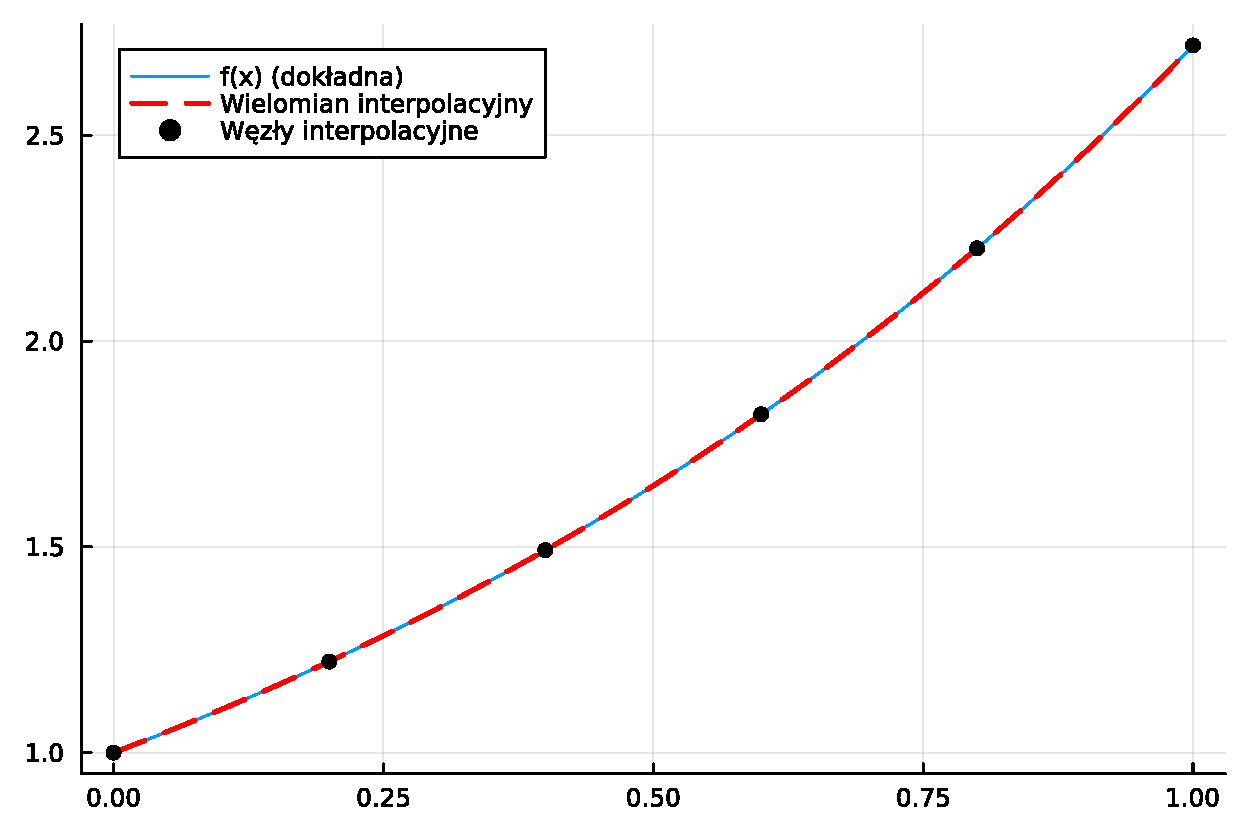
\includegraphics[width=0.7\textwidth, trim = 0 0 0 0, clip]{img/z5_1_5.pdf}
    \caption{Interpolacja funkcji $f(x)=e^x$ dla $n=5$}
\end{figure}


\begin{figure}[H]
    \centering
    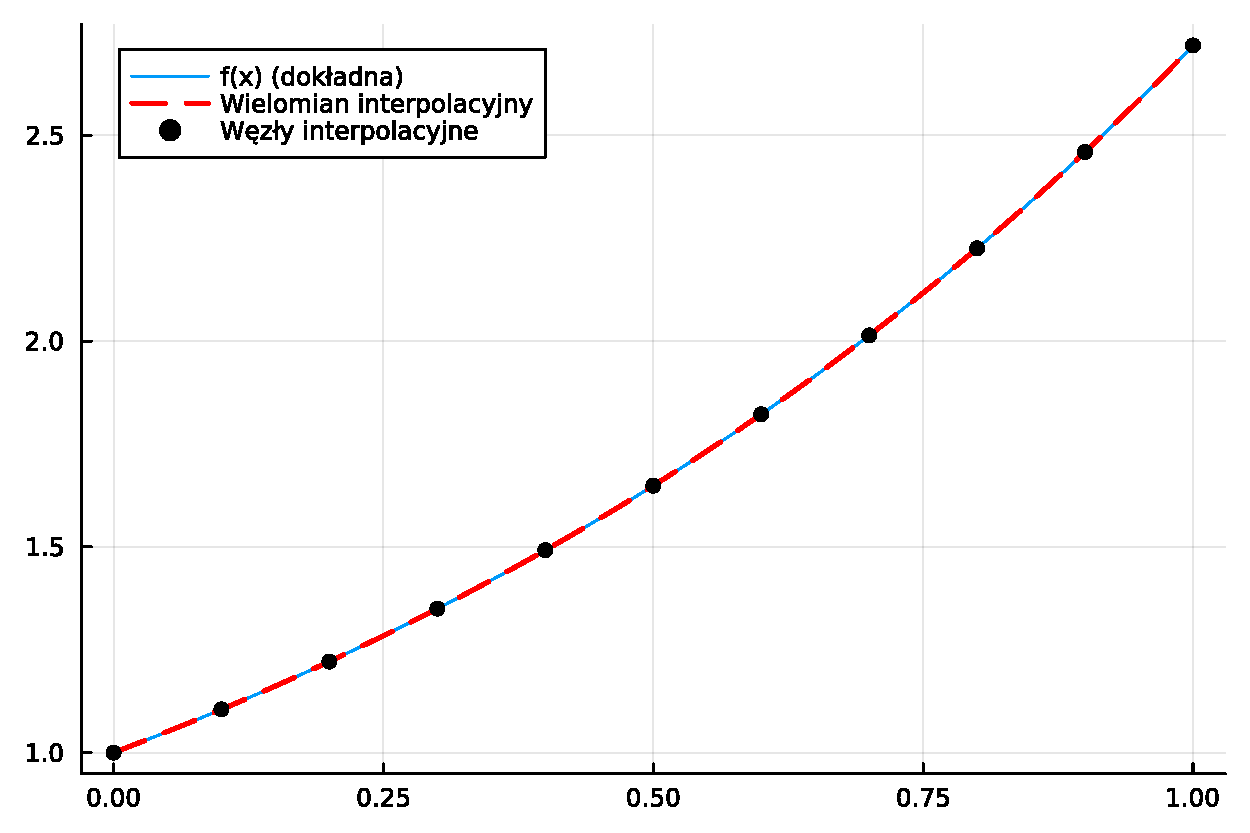
\includegraphics[width=0.7\textwidth, trim = 0 0 0 0, clip]{img/z5_1_10.pdf}
    \caption{Interpolacja funkcji $f(x)=e^x$ dla $n=10$}
\end{figure}


\begin{figure}[H]
    \centering
    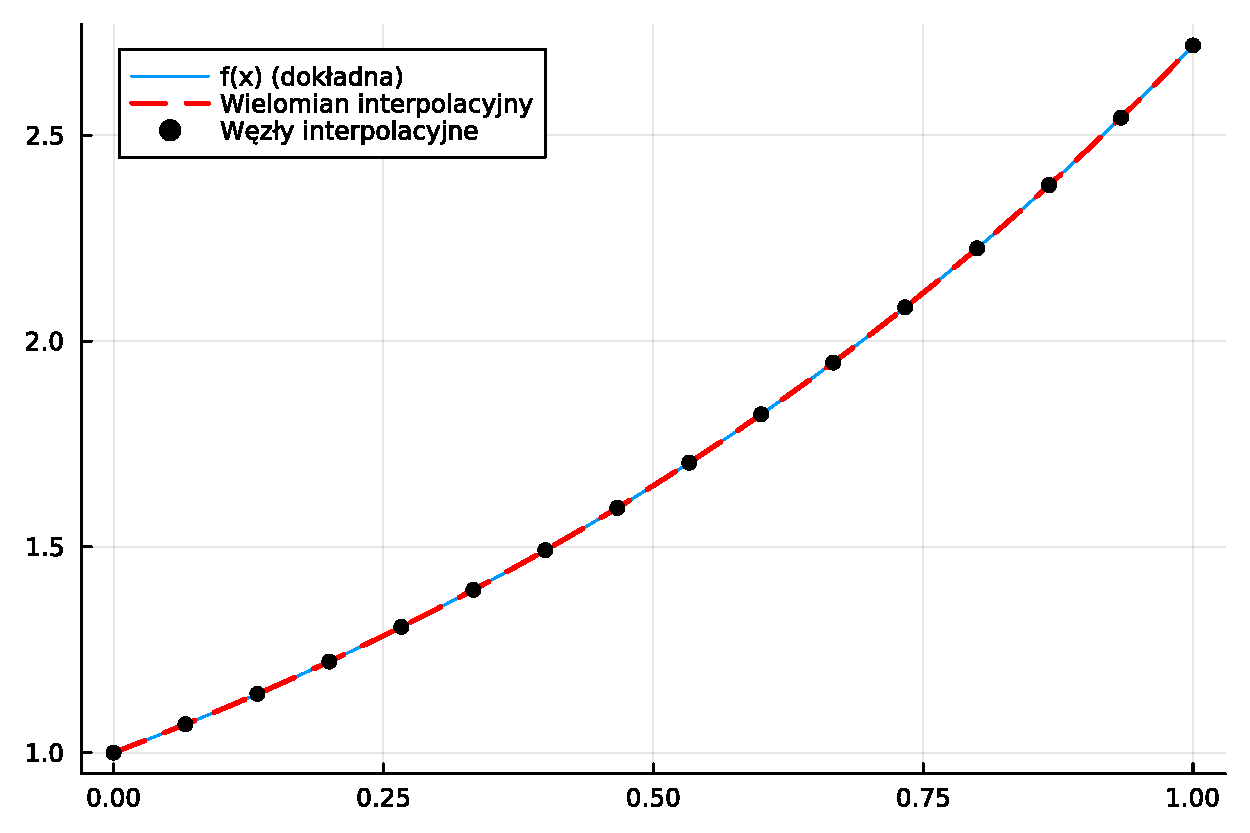
\includegraphics[width=0.7\textwidth, trim = 0 0 0 0, clip]{img/z5_1_15.pdf}
    \caption{Interpolacja funkcji $f(x)=e^x$ dla $n=15$}
\end{figure}
\subsubsection*{Podpunkt 2}
\begin{figure}[H]
    \centering
    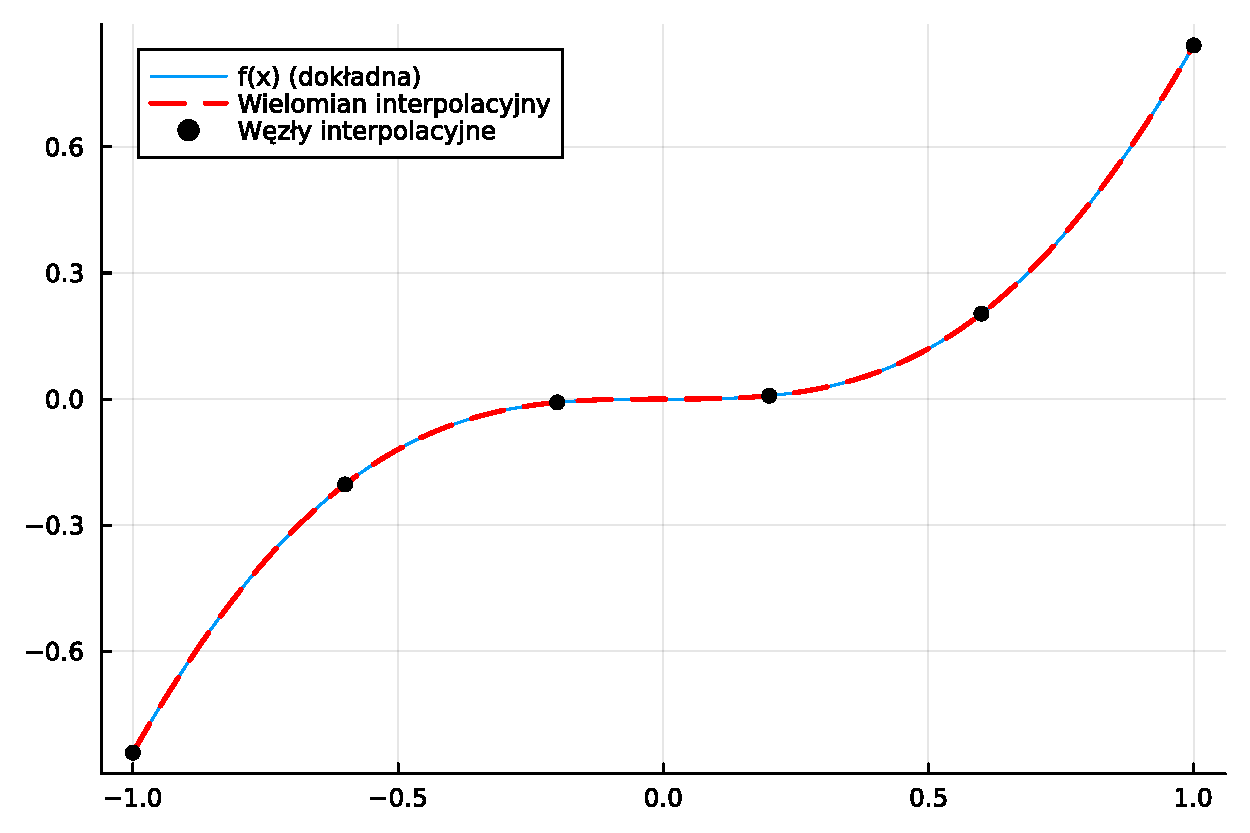
\includegraphics[width=0.7\textwidth, trim = 0 0 0 0, clip]{img/z5_2_5.pdf}
    \caption{Interpolacja funkcji $f(x)=x^2*sin(x)$ dla $n=5$}
\end{figure}


\begin{figure}[H]
    \centering
    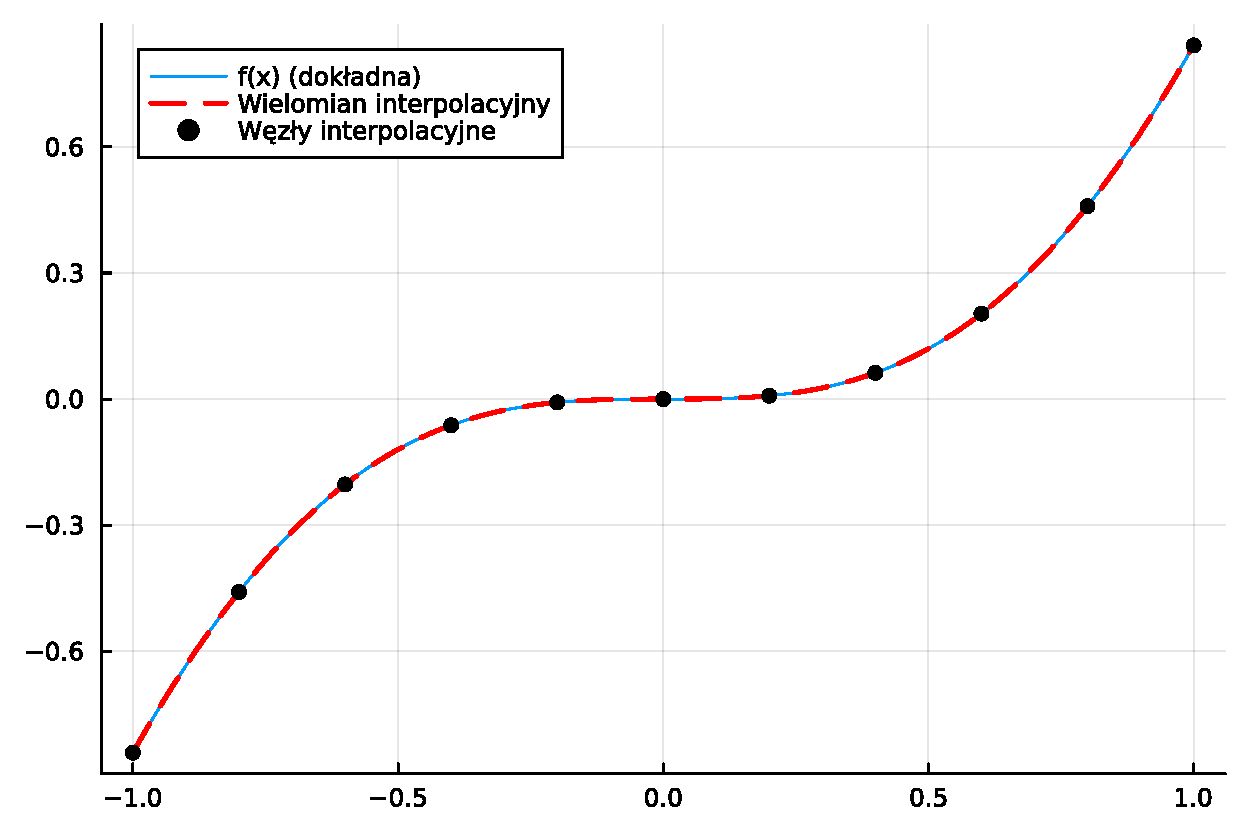
\includegraphics[width=0.7\textwidth, trim = 0 0 0 0, clip]{img/z5_2_10.pdf}
    \caption{Interpolacja funkcji $f(x)=x^2*sin(x)$ dla $n=10$}
\end{figure}


\begin{figure}[H]
    \centering
    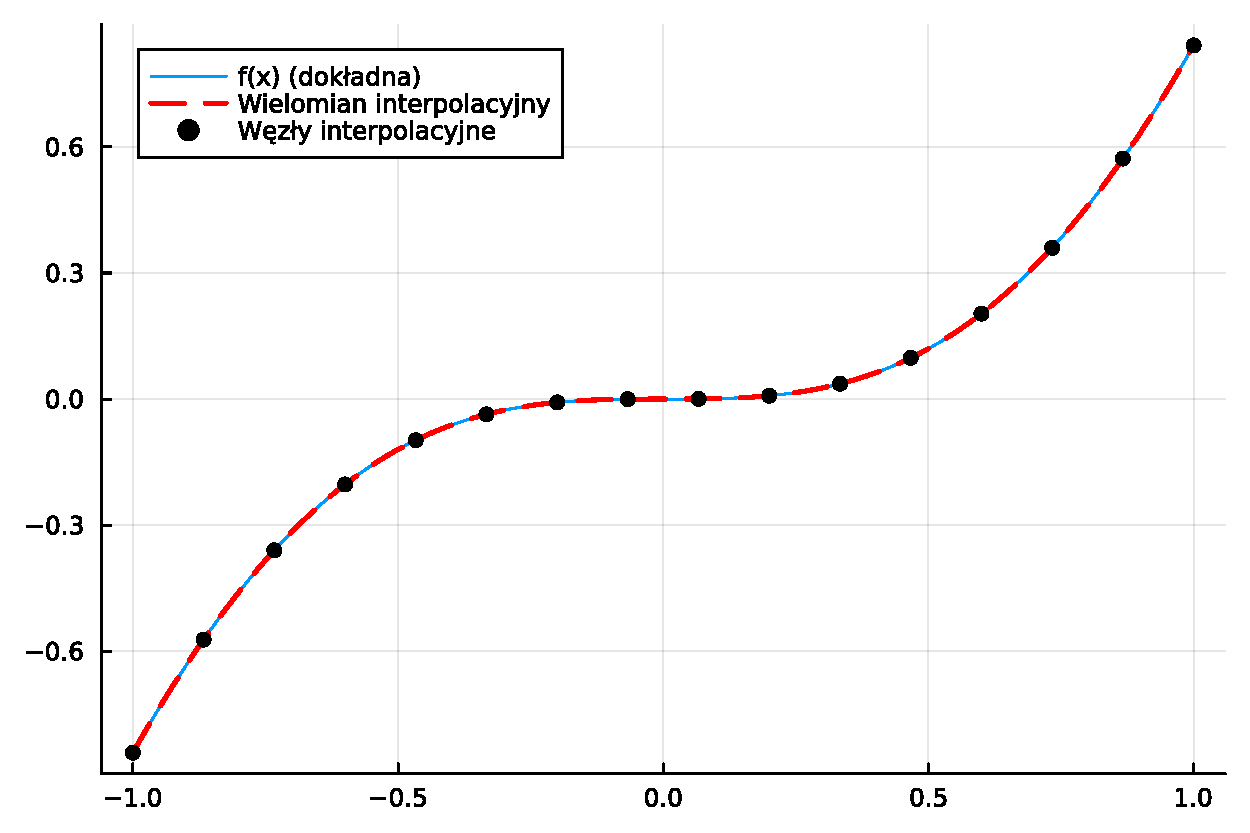
\includegraphics[width=0.7\textwidth, trim = 0 0 0 0, clip]{img/z5_2_15.pdf}
    \caption{Interpolacja funkcji $f(x)=x^2*sin(x)$ dla $n=15$}
\end{figure}
\subsubsection*{Interpretacja}
Wielomiany interpolujące pokrywają się z podanymi funkcjami na wykresach. Wynika to z faktu, że funkcje te są ciągłe oraz gładkie czyli wszystkie ich pochodne także są ciągłe. Dzięki zwiększeniu $n$ błąd interpolacji spada. Błędy tych samych rzędów wychodzą dla wszystkich punktów w przedziale interpolacji.
\subsection*{Wnioski}
Wielomiany interpolujące w bardzo dobry sposób przybliżają funkcje ciągłe, gładkie, różniczkowalne z dobrze zachowującą się pochodną na zadanym przedziale.
\section*{Zadanie 6}
\subsection*{Opis zadania}
Przetestować funkcję \texttt{rysujNnfx(f,a,b,n)} na następujących przykładach (zjawisko rozbieżności):
    \begin{itemize}
        \item $|x|$, $[ −1, 1]$ , $n = 5, 10, 15$
        \item $\frac{1}{1+x^2}$, $[ −5, 5]$ , $n = 5, 10, 15$ (zjawisko Runge’go)
    \end{itemize}
\subsection*{Wyniki i interpretacja}
\subsubsection*{Podpunkt 1}
\begin{figure}[H]
    \centering
    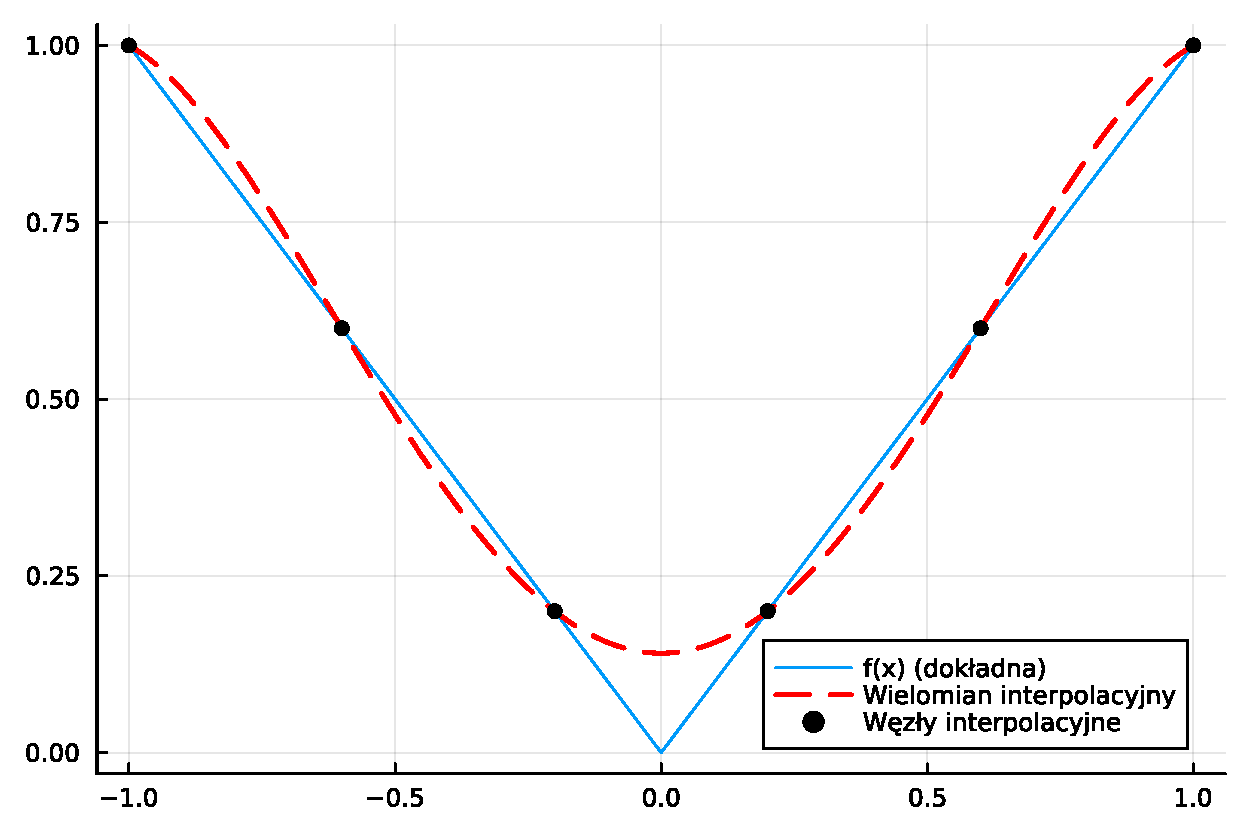
\includegraphics[width=0.7\textwidth, trim = 0 0 0 0, clip]{img/z6_1_5.pdf}
    \caption{Interpolacja funkcji $f(x)=|x|$ dla $n=5$}
\end{figure}

\begin{figure}[H]
    \centering
    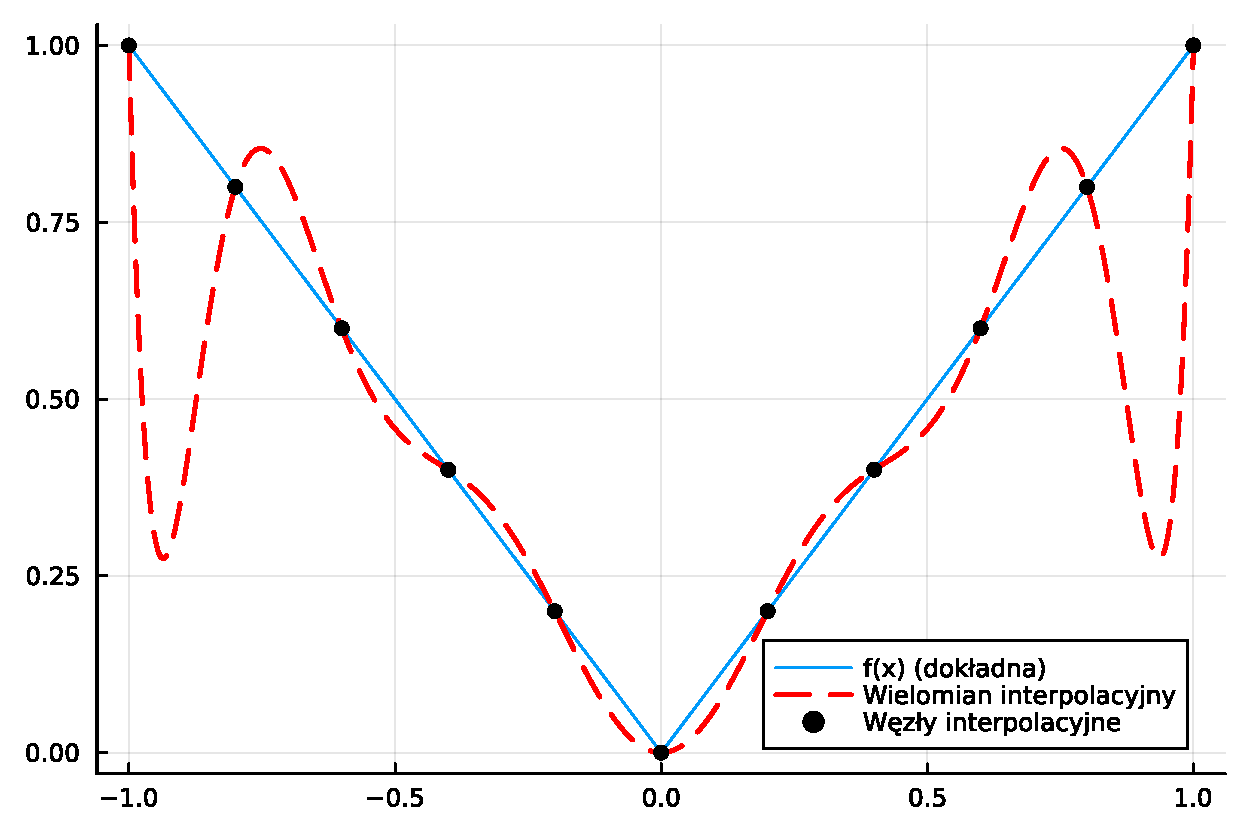
\includegraphics[width=0.7\textwidth, trim = 0 0 0 0, clip]{img/z6_1_10.pdf}
    \caption{Interpolacja funkcji $f(x)=|x|$ dla $n=10$}
\end{figure}

\begin{figure}[H]
    \centering
    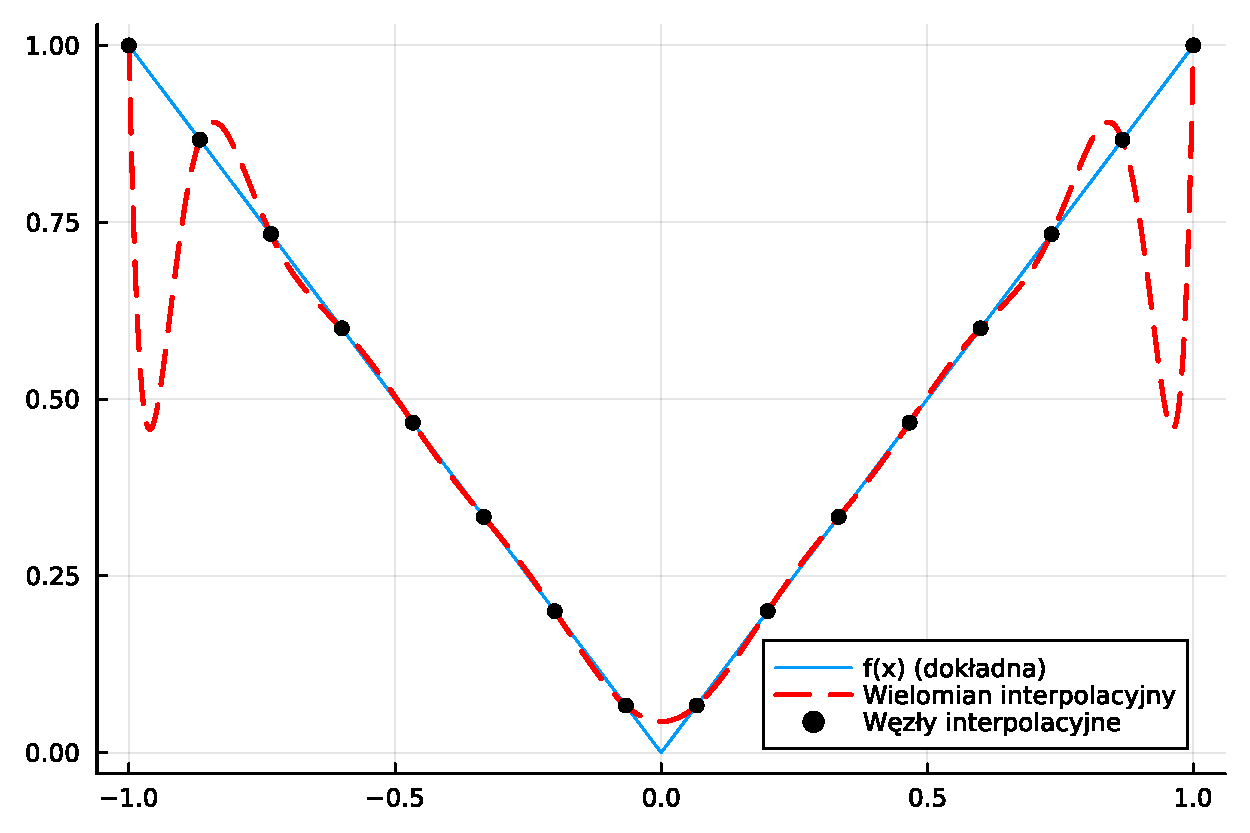
\includegraphics[width=0.7\textwidth, trim = 0 0 0 0, clip]{img/z6_1_15.pdf}
    \caption{Interpolacja funkcji $f(x)=|x|$ dla $n=15$}
\end{figure}
\subsubsection*{Podpunkt 2}
\begin{figure}[H]
    \centering
    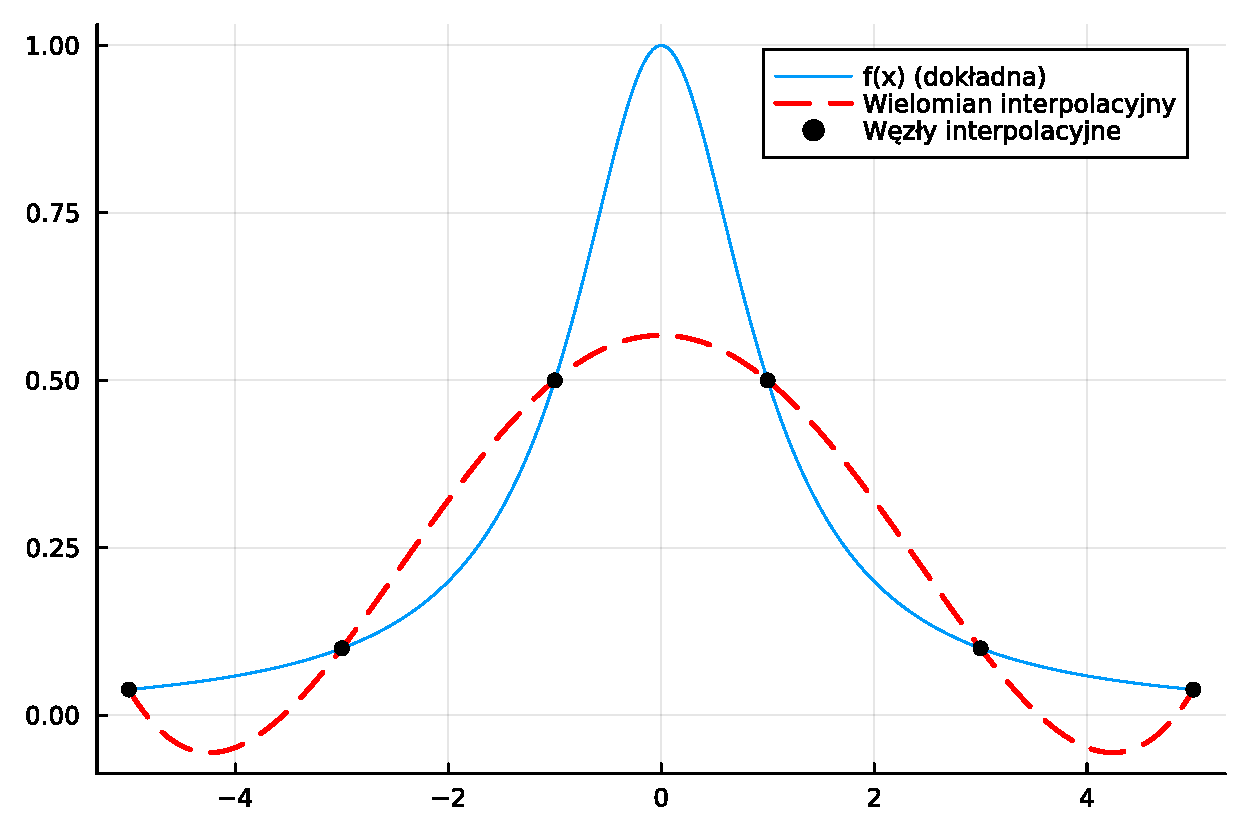
\includegraphics[width=0.7\textwidth, trim = 0 0 0 0, clip]{img/z6_2_5.pdf}
    \caption{Interpolacja funkcji $f(x)=\frac{1}{1+x^2}$ dla $n=5$}
\end{figure}

\begin{figure}[H]
    \centering
    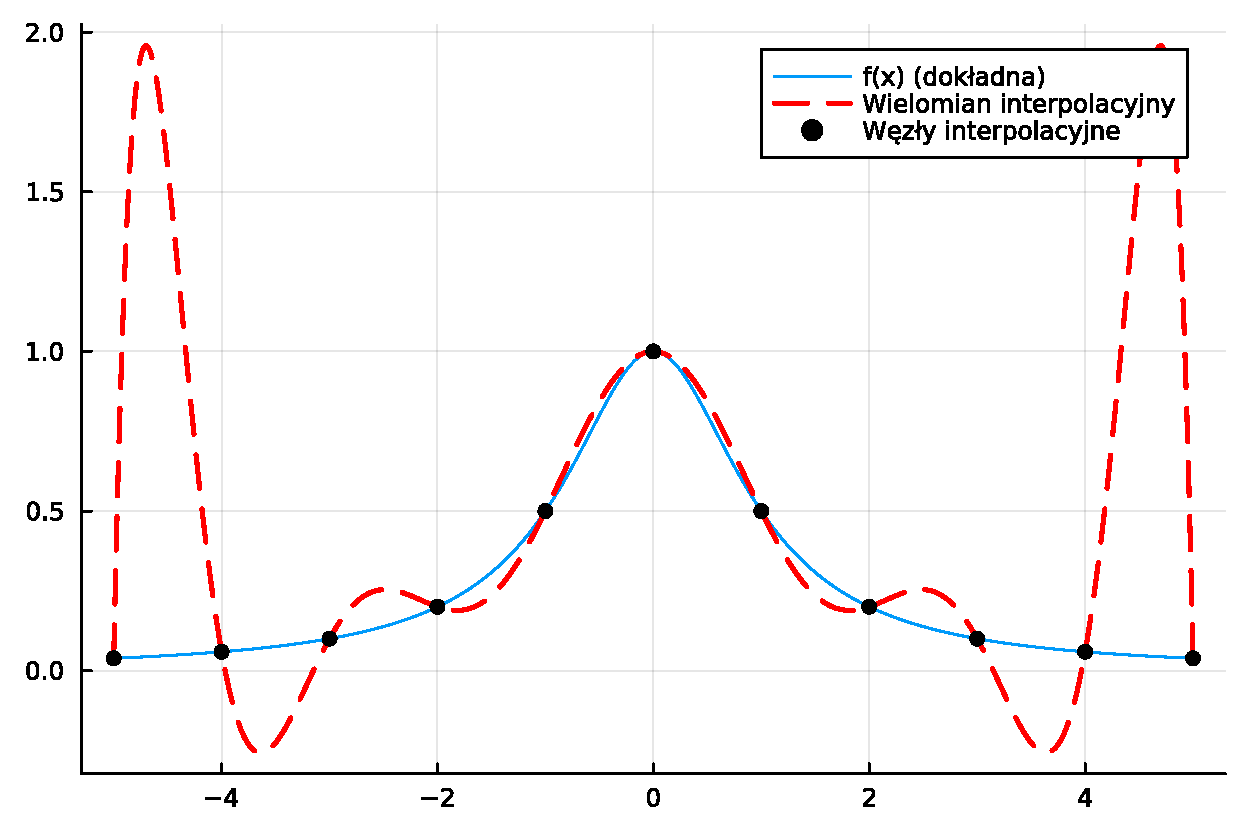
\includegraphics[width=0.7\textwidth, trim = 0 0 0 0, clip]{img/z6_2_10.pdf}
    \caption{Interpolacja funkcji $f(x)=\frac{1}{1+x^2}$ dla $n=10$}
\end{figure}

\begin{figure}[H]
    \centering
    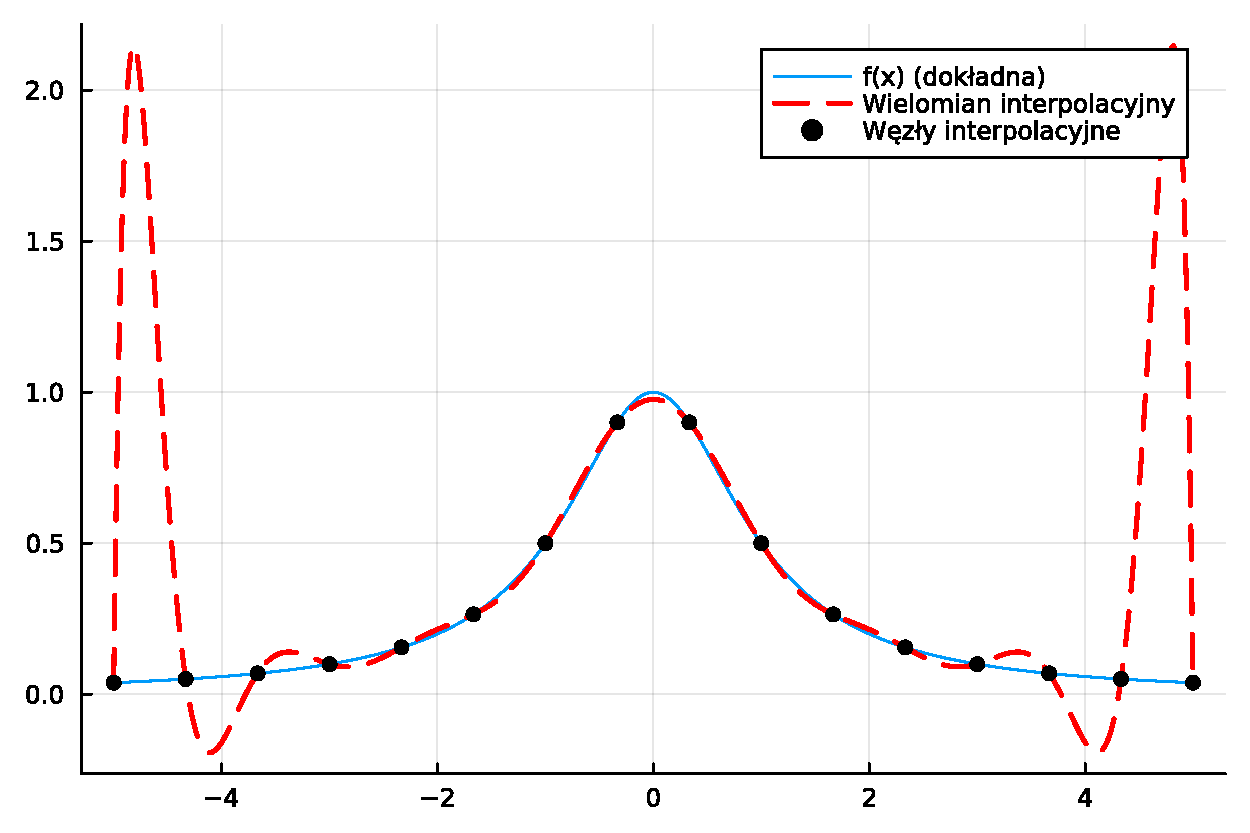
\includegraphics[width=0.7\textwidth, trim = 0 0 0 0, clip]{img/z6_2_15.pdf}
    \caption{Interpolacja funkcji $f(x)=\frac{1}{1+x^2}$ dla $n=15$}
\end{figure}
\subsubsection*{Interpretacja}
Wielomiany interpolacyjne w tym zadaniu bardzo słabo przybliżają zadane funkcje. Zwiększenie liczby punktów interpolujących na danym przedziale poprawia jedynie środkową część wykresu. Jednocześnie pogarsza to przybliżenia na końcach przedziałów. Jest to zjawisko Runge’go. Wynika to z zmiany znaku pochodnej na badanych przedziałach. Problemem jest także równa odległość pomiędzy punktami.
\subsection*{Wnioski}
Aby poprawić wyniki przybliżeń w tym zadaniu należy zagęścić punkty na końcach przedziałów. Jednym z rozwiązań problemu jest użycie do przybliżeń wielomianów węzłów Czebyszewa, które mają więcej węzłów na końcach przedziałów.
\end{document}
